\begin{figure}[htbp]
    \centering
    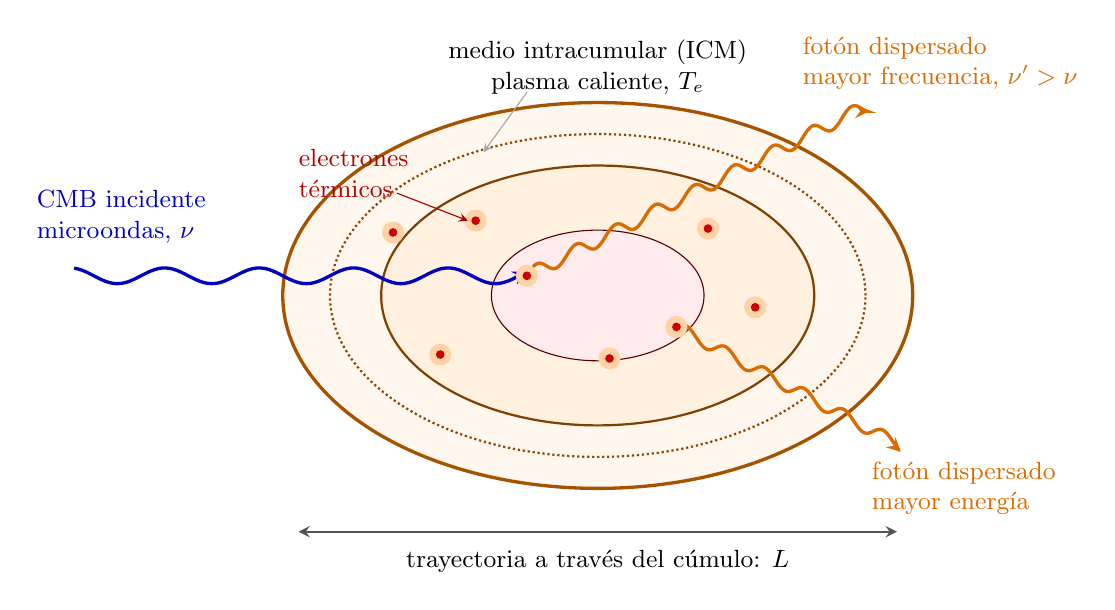
\begin{tikzpicture}[>=stealth, every node/.style={font=\small}]
        \draw[fill=orange!7,draw=orange!65!black,very thick] (7,0) ellipse (4.0cm and 2.45cm);
        \draw[fill=orange!12,draw=orange!50!black,thick] (7,0) ellipse (2.75cm and 1.65cm);
        \draw[fill=red!8,draw=red!35!black] (7,0) ellipse (1.35cm and 0.83cm);
        \draw[orange!55!black,densely dotted,thick] (7,0) ellipse (3.4cm and 2.05cm);

        \node[align=center] at (7,2.9) {medio intracumular (ICM)\\plasma caliente, $T_e$};
        \draw[->,gray!70,thin] (6.1,2.58) -- (5.55,1.82);

        \draw[->,very thick,blue!75!black,domain=0.35:6.1,samples=120,smooth]
            plot (\x,{0.25+0.10*sin(300*\x)});
        \draw[->,very thick,orange!85!black,domain=6.1:10.45,samples=140,smooth]
            plot (\x,{0.25+0.50*(\x-6.1)+0.09*sin(720*(\x-6.1))});
        \draw[->,very thick,orange!85!black,domain=8.0:10.85,samples=120,smooth]
            plot (\x,{-0.4-0.53*(\x-8.0)+0.08*sin(720*(\x-8.0))});

        \foreach \x/\y in {4.4/0.8,5.0/-0.75,5.45/0.95,6.1/0.25,7.15/-0.8,8.0/-0.4,8.4/0.85,9.0/-0.15}
        {
            \fill[orange!35] (\x,\y) circle (0.14);
            \fill[red!80!black] (\x,\y) circle (0.055);
        }
        \node[red!70!black,align=left] at (3.9,1.55) {electrones\\térmicos};
        \draw[->,red!65!black] (4.45,1.3) -- (5.35,0.95);

        \node[blue!75!black,align=left] at (0.95,1.0) {CMB incidente\\microondas, $\nu$};
        \node[orange!85!black,align=left] at (11.35,2.95)
            {fotón dispersado\\mayor frecuencia, $\nu'>\nu$};
        \node[orange!85!black,align=left] at (11.65,-2.45)
            {fotón dispersado\\mayor energía};

        \draw[<->,gray!65!black,thick] (3.2,-3.0) -- (10.8,-3.0)
            node[midway,below=3pt,text=black] {trayectoria a través del cúmulo: $L$};
    \end{tikzpicture}
    \caption{Esquema del efecto Sunyaev--Zel'dovich térmico: los fotones de baja energía del CMB atraviesan el ICM y, al dispersarse con electrones calientes, ganan energía. La intensidad del efecto depende del parámetro $y=(k_BT_e/m_ec^2)\,\sigma_T\int n_e\,d\ell$.}
    \label{fig:efecto-sz}
\end{figure}